\documentclass[border=4pt]{standalone}

\usepackage{amsmath}
\usepackage{tikz}
\usepackage{mathdots}
\usepackage{yhmath}
\usepackage{cancel}
\usepackage{color}
\usepackage{siunitx}
\usepackage{array}
\usepackage{multirow}
\usepackage{amssymb}
\usepackage{gensymb}
\usepackage{tabularx}
\usepackage{booktabs}
\usetikzlibrary{fadings}
\usetikzlibrary{patterns}


\begin{document}
 
     



\tikzset{every picture/.style={line width=0.75pt}} %set default line width to 0.75pt        

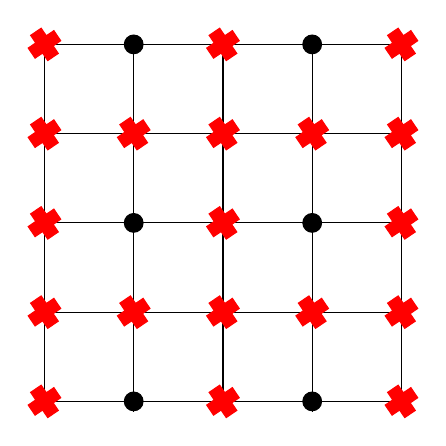
\begin{tikzpicture}[x=0.75pt,y=0.75pt,yscale=-1,xscale=1]
%uncomment if require: \path (0,300); %set diagram left start at 0, and has height of 300

%Shape: Grid [id:dp9074145679501431] 
\draw  [draw opacity=0] (180,70) -- (356.18,70) -- (356.18,247) -- (180,247) -- cycle ; \draw   (180,70) -- (180,247)(223,70) -- (223,247)(266,70) -- (266,247)(309,70) -- (309,247)(352,70) -- (352,247) ; \draw   (180,70) -- (356.18,70)(180,113) -- (356.18,113)(180,156) -- (356.18,156)(180,199) -- (356.18,199)(180,242) -- (356.18,242) ; \draw    ;
%Shape: Circle [id:dp058548282299102805] 
\draw  [color={rgb, 255:red, 0; green, 0; blue, 0 }  ,draw opacity=1 ][fill={rgb, 255:red, 0; green, 0; blue, 0 }  ,fill opacity=1 ] (218.5,70) .. controls (218.5,67.51) and (220.51,65.5) .. (223,65.5) .. controls (225.49,65.5) and (227.5,67.51) .. (227.5,70) .. controls (227.5,72.49) and (225.49,74.5) .. (223,74.5) .. controls (220.51,74.5) and (218.5,72.49) .. (218.5,70) -- cycle ;
%Shape: Circle [id:dp1719878871313243] 
\draw  [color={rgb, 255:red, 0; green, 0; blue, 0 }  ,draw opacity=1 ][fill={rgb, 255:red, 0; green, 0; blue, 0 }  ,fill opacity=1 ] (218.5,156) .. controls (218.5,153.51) and (220.51,151.5) .. (223,151.5) .. controls (225.49,151.5) and (227.5,153.51) .. (227.5,156) .. controls (227.5,158.49) and (225.49,160.5) .. (223,160.5) .. controls (220.51,160.5) and (218.5,158.49) .. (218.5,156) -- cycle ;
%Shape: Circle [id:dp3364777633556906] 
\draw  [color={rgb, 255:red, 0; green, 0; blue, 0 }  ,draw opacity=1 ][fill={rgb, 255:red, 0; green, 0; blue, 0 }  ,fill opacity=1 ] (218.5,242) .. controls (218.5,239.51) and (220.51,237.5) .. (223,237.5) .. controls (225.49,237.5) and (227.5,239.51) .. (227.5,242) .. controls (227.5,244.49) and (225.49,246.5) .. (223,246.5) .. controls (220.51,246.5) and (218.5,244.49) .. (218.5,242) -- cycle ;
%Shape: Circle [id:dp4738566045287167] 
\draw  [color={rgb, 255:red, 0; green, 0; blue, 0 }  ,draw opacity=1 ][fill={rgb, 255:red, 0; green, 0; blue, 0 }  ,fill opacity=1 ] (304.5,242) .. controls (304.5,239.51) and (306.51,237.5) .. (309,237.5) .. controls (311.49,237.5) and (313.5,239.51) .. (313.5,242) .. controls (313.5,244.49) and (311.49,246.5) .. (309,246.5) .. controls (306.51,246.5) and (304.5,244.49) .. (304.5,242) -- cycle ;
%Shape: Circle [id:dp715970197171246] 
\draw  [color={rgb, 255:red, 0; green, 0; blue, 0 }  ,draw opacity=1 ][fill={rgb, 255:red, 0; green, 0; blue, 0 }  ,fill opacity=1 ] (304.5,156) .. controls (304.5,153.51) and (306.51,151.5) .. (309,151.5) .. controls (311.49,151.5) and (313.5,153.51) .. (313.5,156) .. controls (313.5,158.49) and (311.49,160.5) .. (309,160.5) .. controls (306.51,160.5) and (304.5,158.49) .. (304.5,156) -- cycle ;
%Shape: Circle [id:dp4034686585002938] 
\draw  [color={rgb, 255:red, 0; green, 0; blue, 0 }  ,draw opacity=1 ][fill={rgb, 255:red, 0; green, 0; blue, 0 }  ,fill opacity=1 ] (304.5,70) .. controls (304.5,67.51) and (306.51,65.5) .. (309,65.5) .. controls (311.49,65.5) and (313.5,67.51) .. (313.5,70) .. controls (313.5,72.49) and (311.49,74.5) .. (309,74.5) .. controls (306.51,74.5) and (304.5,72.49) .. (304.5,70) -- cycle ;
%Shape: Cross [id:dp7539299936054427] 
\draw  [color={rgb, 255:red, 255; green, 0; blue, 0 }  ,draw opacity=1 ][fill={rgb, 255:red, 255; green, 0; blue, 0 }  ,fill opacity=1 ] (184.53,63.38) -- (187.82,68.24) -- (184.18,70.71) -- (186.65,74.35) -- (181.58,77.79) -- (179.11,74.15) -- (175.47,76.62) -- (172.18,71.76) -- (175.82,69.29) -- (173.35,65.65) -- (178.42,62.21) -- (180.89,65.85) -- cycle ;
%Shape: Cross [id:dp27704668754942396] 
\draw  [color={rgb, 255:red, 255; green, 0; blue, 0 }  ,draw opacity=1 ][fill={rgb, 255:red, 255; green, 0; blue, 0 }  ,fill opacity=1 ] (227.53,106.38) -- (230.82,111.24) -- (227.18,113.71) -- (229.65,117.35) -- (224.58,120.79) -- (222.11,117.15) -- (218.47,119.62) -- (215.18,114.76) -- (218.82,112.29) -- (216.35,108.65) -- (221.42,105.21) -- (223.89,108.85) -- cycle ;
%Shape: Cross [id:dp841214098113996] 
\draw  [color={rgb, 255:red, 255; green, 0; blue, 0 }  ,draw opacity=1 ][fill={rgb, 255:red, 255; green, 0; blue, 0 }  ,fill opacity=1 ] (184.53,149.38) -- (187.82,154.24) -- (184.18,156.71) -- (186.65,160.35) -- (181.58,163.79) -- (179.11,160.15) -- (175.47,162.62) -- (172.18,157.76) -- (175.82,155.29) -- (173.35,151.65) -- (178.42,148.21) -- (180.89,151.85) -- cycle ;
%Shape: Cross [id:dp8491021865470889] 
\draw  [color={rgb, 255:red, 255; green, 0; blue, 0 }  ,draw opacity=1 ][fill={rgb, 255:red, 255; green, 0; blue, 0 }  ,fill opacity=1 ] (270.53,63.38) -- (273.82,68.24) -- (270.18,70.71) -- (272.65,74.35) -- (267.58,77.79) -- (265.11,74.15) -- (261.47,76.62) -- (258.18,71.76) -- (261.82,69.29) -- (259.35,65.65) -- (264.42,62.21) -- (266.89,65.85) -- cycle ;
%Shape: Cross [id:dp18327633111257047] 
\draw  [color={rgb, 255:red, 255; green, 0; blue, 0 }  ,draw opacity=1 ][fill={rgb, 255:red, 255; green, 0; blue, 0 }  ,fill opacity=1 ] (227.53,192.38) -- (230.82,197.24) -- (227.18,199.71) -- (229.65,203.35) -- (224.58,206.79) -- (222.11,203.15) -- (218.47,205.62) -- (215.18,200.76) -- (218.82,198.29) -- (216.35,194.65) -- (221.42,191.21) -- (223.89,194.85) -- cycle ;
%Shape: Cross [id:dp8079603335794479] 
\draw  [color={rgb, 255:red, 255; green, 0; blue, 0 }  ,draw opacity=1 ][fill={rgb, 255:red, 255; green, 0; blue, 0 }  ,fill opacity=1 ] (270.53,149.38) -- (273.82,154.24) -- (270.18,156.71) -- (272.65,160.35) -- (267.58,163.79) -- (265.11,160.15) -- (261.47,162.62) -- (258.18,157.76) -- (261.82,155.29) -- (259.35,151.65) -- (264.42,148.21) -- (266.89,151.85) -- cycle ;
%Shape: Cross [id:dp4804845300169138] 
\draw  [color={rgb, 255:red, 255; green, 0; blue, 0 }  ,draw opacity=1 ][fill={rgb, 255:red, 255; green, 0; blue, 0 }  ,fill opacity=1 ] (313.53,106.38) -- (316.82,111.24) -- (313.18,113.71) -- (315.65,117.35) -- (310.58,120.79) -- (308.11,117.15) -- (304.47,119.62) -- (301.18,114.76) -- (304.82,112.29) -- (302.35,108.65) -- (307.42,105.21) -- (309.89,108.85) -- cycle ;
%Shape: Cross [id:dp43450513664161683] 
\draw  [color={rgb, 255:red, 255; green, 0; blue, 0 }  ,draw opacity=1 ][fill={rgb, 255:red, 255; green, 0; blue, 0 }  ,fill opacity=1 ] (313.53,192.38) -- (316.82,197.24) -- (313.18,199.71) -- (315.65,203.35) -- (310.58,206.79) -- (308.11,203.15) -- (304.47,205.62) -- (301.18,200.76) -- (304.82,198.29) -- (302.35,194.65) -- (307.42,191.21) -- (309.89,194.85) -- cycle ;
%Shape: Cross [id:dp1938076077056572] 
\draw  [color={rgb, 255:red, 255; green, 0; blue, 0 }  ,draw opacity=1 ][fill={rgb, 255:red, 255; green, 0; blue, 0 }  ,fill opacity=1 ] (184.53,106.38) -- (187.82,111.24) -- (184.18,113.71) -- (186.65,117.35) -- (181.58,120.79) -- (179.11,117.15) -- (175.47,119.62) -- (172.18,114.76) -- (175.82,112.29) -- (173.35,108.65) -- (178.42,105.21) -- (180.89,108.85) -- cycle ;
%Shape: Cross [id:dp6202530351602755] 
\draw  [color={rgb, 255:red, 255; green, 0; blue, 0 }  ,draw opacity=1 ][fill={rgb, 255:red, 255; green, 0; blue, 0 }  ,fill opacity=1 ] (184.53,192.38) -- (187.82,197.24) -- (184.18,199.71) -- (186.65,203.35) -- (181.58,206.79) -- (179.11,203.15) -- (175.47,205.62) -- (172.18,200.76) -- (175.82,198.29) -- (173.35,194.65) -- (178.42,191.21) -- (180.89,194.85) -- cycle ;
%Shape: Cross [id:dp2802141458635423] 
\draw  [color={rgb, 255:red, 255; green, 0; blue, 0 }  ,draw opacity=1 ][fill={rgb, 255:red, 255; green, 0; blue, 0 }  ,fill opacity=1 ] (184.53,235.38) -- (187.82,240.24) -- (184.18,242.71) -- (186.65,246.35) -- (181.58,249.79) -- (179.11,246.15) -- (175.47,248.62) -- (172.18,243.76) -- (175.82,241.29) -- (173.35,237.65) -- (178.42,234.21) -- (180.89,237.85) -- cycle ;
%Shape: Cross [id:dp057542650266022566] 
\draw  [color={rgb, 255:red, 255; green, 0; blue, 0 }  ,draw opacity=1 ][fill={rgb, 255:red, 255; green, 0; blue, 0 }  ,fill opacity=1 ] (270.53,106.38) -- (273.82,111.24) -- (270.18,113.71) -- (272.65,117.35) -- (267.58,120.79) -- (265.11,117.15) -- (261.47,119.62) -- (258.18,114.76) -- (261.82,112.29) -- (259.35,108.65) -- (264.42,105.21) -- (266.89,108.85) -- cycle ;
%Shape: Cross [id:dp3443173468909615] 
\draw  [color={rgb, 255:red, 255; green, 0; blue, 0 }  ,draw opacity=1 ][fill={rgb, 255:red, 255; green, 0; blue, 0 }  ,fill opacity=1 ] (270.53,235.38) -- (273.82,240.24) -- (270.18,242.71) -- (272.65,246.35) -- (267.58,249.79) -- (265.11,246.15) -- (261.47,248.62) -- (258.18,243.76) -- (261.82,241.29) -- (259.35,237.65) -- (264.42,234.21) -- (266.89,237.85) -- cycle ;
%Shape: Cross [id:dp12730987108638203] 
\draw  [color={rgb, 255:red, 255; green, 0; blue, 0 }  ,draw opacity=1 ][fill={rgb, 255:red, 255; green, 0; blue, 0 }  ,fill opacity=1 ] (270.53,192.38) -- (273.82,197.24) -- (270.18,199.71) -- (272.65,203.35) -- (267.58,206.79) -- (265.11,203.15) -- (261.47,205.62) -- (258.18,200.76) -- (261.82,198.29) -- (259.35,194.65) -- (264.42,191.21) -- (266.89,194.85) -- cycle ;
%Shape: Cross [id:dp03371921076744444] 
\draw  [color={rgb, 255:red, 255; green, 0; blue, 0 }  ,draw opacity=1 ][fill={rgb, 255:red, 255; green, 0; blue, 0 }  ,fill opacity=1 ] (356.53,192.38) -- (359.82,197.24) -- (356.18,199.71) -- (358.65,203.35) -- (353.58,206.79) -- (351.11,203.15) -- (347.47,205.62) -- (344.18,200.76) -- (347.82,198.29) -- (345.35,194.65) -- (350.42,191.21) -- (352.89,194.85) -- cycle ;
%Shape: Cross [id:dp5138543158482227] 
\draw  [color={rgb, 255:red, 255; green, 0; blue, 0 }  ,draw opacity=1 ][fill={rgb, 255:red, 255; green, 0; blue, 0 }  ,fill opacity=1 ] (356.53,149.38) -- (359.82,154.24) -- (356.18,156.71) -- (358.65,160.35) -- (353.58,163.79) -- (351.11,160.15) -- (347.47,162.62) -- (344.18,157.76) -- (347.82,155.29) -- (345.35,151.65) -- (350.42,148.21) -- (352.89,151.85) -- cycle ;
%Shape: Cross [id:dp8721132317272153] 
\draw  [color={rgb, 255:red, 255; green, 0; blue, 0 }  ,draw opacity=1 ][fill={rgb, 255:red, 255; green, 0; blue, 0 }  ,fill opacity=1 ] (356.53,106.38) -- (359.82,111.24) -- (356.18,113.71) -- (358.65,117.35) -- (353.58,120.79) -- (351.11,117.15) -- (347.47,119.62) -- (344.18,114.76) -- (347.82,112.29) -- (345.35,108.65) -- (350.42,105.21) -- (352.89,108.85) -- cycle ;
%Shape: Cross [id:dp7486643026750202] 
\draw  [color={rgb, 255:red, 255; green, 0; blue, 0 }  ,draw opacity=1 ][fill={rgb, 255:red, 255; green, 0; blue, 0 }  ,fill opacity=1 ] (356.53,63.38) -- (359.82,68.24) -- (356.18,70.71) -- (358.65,74.35) -- (353.58,77.79) -- (351.11,74.15) -- (347.47,76.62) -- (344.18,71.76) -- (347.82,69.29) -- (345.35,65.65) -- (350.42,62.21) -- (352.89,65.85) -- cycle ;
%Shape: Cross [id:dp7442170494561329] 
\draw  [color={rgb, 255:red, 255; green, 0; blue, 0 }  ,draw opacity=1 ][fill={rgb, 255:red, 255; green, 0; blue, 0 }  ,fill opacity=1 ] (356.53,235.38) -- (359.82,240.24) -- (356.18,242.71) -- (358.65,246.35) -- (353.58,249.79) -- (351.11,246.15) -- (347.47,248.62) -- (344.18,243.76) -- (347.82,241.29) -- (345.35,237.65) -- (350.42,234.21) -- (352.89,237.85) -- cycle ;




\end{tikzpicture}


\end{document}
